\documentclass[12pt]{article}
\usepackage[utf8]{inputenc}
\usepackage[brazil]{babel}
\usepackage{amsmath, amssymb, array, bm, geometry, booktabs, siunitx, graphicx, colortbl, parskip, xcolor}
\usepackage{listings}
\usepackage{color}
\usepackage{float}
\usepackage{fancyhdr}
\usepackage{titlesec}
\usepackage{hyperref}
\usepackage{listings}

\setlength{\headheight}{14.5pt}
\addtolength{\topmargin}{-2.5pt}
\geometry{a4paper, total={6in, 9in}}




\definecolor{codegray}{gray}{0.9}
\lstset{
    backgroundcolor=\color{codegray},
    basicstyle=\ttfamily\footnotesize,
    frame=single,
    breaklines=true,
    captionpos=b,
    numbers=left,
    numberstyle=\tiny,
    language=Python
}

% Cabeçalho
\pagestyle{fancy}
\fancyhf{}
\rhead{UnB}
\lhead{Departamento de Ci\^encias Mec\^anicas}
\cfoot{\thepage}

\titleformat{\section}{\large\bfseries}{\thesection}{1em}{}

\begin{document}

% Capa
\begin{titlepage}
    \centering
    
\includegraphics[width=12cm]{img/unb_bandeira.png} \\
    \vspace{1cm}
    \textsc{\Large Universidade de Bras\'ilia} \\
    \textsc{Departamento de Ciências Mec\^anicas} \\
    \textsc{Programa de P\'os-Gradua\c{c}\~ao} \\
    \vfill
    {\Large\bfseries Programa 7} \\
    \vspace{0.5cm}
    {\Large\bfseries Integração Numérica - Fórmulas Fechadas de Newton-Cotes} \\
    \vspace{0.5cm}
    \textbf{Disciplina: M\'etodos Num\'ericos} \\
    Professor: Dr. Rafael Gabler Gontijo \\
    \vfill
    \textbf{Aluno: Eng. Lucas Wanick — Mestrando em Engenharia Mec\^anica} \\
    \vspace{0.5cm}
        \today \\
\end{titlepage}


\section{Introdução}
O exercício propõe a aplicação de métodos de integração numérica para o cálculo do valor médio de uma função $T(x,y)$ sobre uma malha geométrica $n \times n$, definida no domínio $[0,1]\times[0,1]$. A função considerada neste programa é um polinômio quadrático, o que permite avaliar a precisão dos métodos numéricos em relação à solução analítica obtida pela integração direta.

\begin{equation}
    T(x,y) = 2xy + 2x - x^2 - 2y^2 + 72
\end{equation}

O código desenvolvido incorpora a função $T(x,y)$ e utiliza três métodos distintos de integração numérica: a regra do trapézio, a regra 1/3 de Simpson e a regra 3/8 de Simpson. Os resultados são organizados em tabelas e comparados com o valor exato da integral dupla, a fim de verificar o erro absoluto associado a cada abordagem.

\section{Integração Numérica}

\subsection{Regra de Simpson}

A regra de Simpson baseia-se na aproximação da função $f(x)$ por um polinômio interpolador de Lagrange. A seguir, deduzimos as expressões para as fórmulas conhecidas como Simpson 1/3 e 3/8.

\subsubsection*{Regra de Simpson 1/3 para um único intervalo}

Desejamos deduzir a fórmula de integração numérica conhecida como \textbf{Regra de Simpson 1/3}, baseada na interpolação de Lagrange de segundo grau. Seja \( f(x) \) uma função suficientemente suave em um intervalo \( [x_0, x_2] \), com espaçamento uniforme \( h = \frac{x_2 - x_0}{2} \). Definimos:

\[
x_0 = a, \quad x_1 = a + h, \quad x_2 = a + 2h = b
\]

Interpolamos \( f(x) \) por um polinômio de Lagrange de grau 2:

\[
P_2(x) = f(x_0) \cdot \frac{(x - x_1)(x - x_2)}{(x_0 - x_1)(x_0 - x_2)}
+ f(x_1) \cdot \frac{(x - x_0)(x - x_2)}{(x_1 - x_0)(x_1 - x_2)}
+ f(x_2) \cdot \frac{(x - x_0)(x - x_1)}{(x_2 - x_0)(x_2 - x_1)}
\]

Substituindo os valores dos nós:

\[
\begin{aligned}
P_2(x) = & f(x_0) \cdot \frac{(x - a - h)(x - a - 2h)}{2h^2}
- f(x_1) \cdot \frac{(x - a)(x - a - 2h)}{h^2} \\
& + f(x_2) \cdot \frac{(x - a)(x - a - h)}{2h^2}
\end{aligned}
\]

Fazemos a mudança de variável \( x = a + t \), com \( t \in [0, 2h] \). Assim:

\[
I = \int_a^{a+2h} P_2(x) dx = I_0 + I_1 + I_2
\]

Calculamos separadamente os termos:

\[
I_0 = f(x_0) \cdot \frac{1}{2h^2} \int_0^{2h} (t - h)(t - 2h) dt
= f(x_0) \cdot \frac{1}{2h^2} \int_0^{2h} (t^2 - 3ht + 2h^2) dt
= \frac{h}{3} f(x_0)
\]

\[
I_1 = -f(x_1) \cdot \frac{1}{h^2} \int_0^{2h} t(t - 2h) dt
= -f(x_1) \cdot \frac{1}{h^2} \int_0^{2h} (t^2 - 2ht) dt
= \frac{4h}{3} f(x_1)
\]

\[
I_2 = f(x_2) \cdot \frac{1}{2h^2} \int_0^{2h} t(t - h) dt
= f(x_2) \cdot \frac{1}{2h^2} \int_0^{2h} (t^2 - ht) dt
= \frac{h}{3} f(x_2)
\]

Somando os três termos:

\[
I \approx \int_{x_0}^{x_2} f(x) dx \approx \frac{h}{3} \left[ f(x_0) + 4f(x_1) + f(x_2) \right]
\]

Essa é a \textbf{Regra de Simpson 1/3}, também conhecida como fórmula fechada de Newton-Cotes de segundo grau.

\subsubsection*{Regra de Simpson 1/3 para múltiplos intervalos}

Seja o intervalo $[a, b]$ dividido em $n$ subintervalos de largura $h = (b - a)/n$, onde $n$ é um número **par**. Aplicando a Regra de Simpson 1/3 a cada par de subintervalos, temos:

\[
\int_a^b f(x)\,dx \approx \sum_{i=0}^{n/2 - 1} \int_{x_{2i}}^{x_{2i+2}} f(x)\,dx
\]

Para cada par de subintervalos $[x_{2i}, x_{2i+2}]$, usamos a Regra de Simpson 1/3:

\[
\int_{x_{2i}}^{x_{2i+2}} f(x)\,dx \approx \frac{h}{3} \left[f(x_{2i}) + 4f(x_{2i+1}) + f(x_{2i+2})\right]
\]

Somando todas essas contribuições:

\[
\int_a^b f(x)\,dx \approx \frac{h}{3} \left[f(x_0) + 4f(x_1) + 2f(x_2) + 4f(x_3) + 2f(x_4) + \dots + 4f(x_{n-1}) + f(x_n)\right]
\]

Reescrevendo a expressão de forma condensada:

\[
\int_a^b f(x)\,dx \approx \frac{h}{3} \left[
f(x_0) + f(x_n)
+ 4 \sum_{\substack{i = 1 \\ i\ \text{ímpar}}}^{n-1} f(x_i)
+ 2 \sum_{\substack{j = 2 \\ j\ \text{par}}}^{n-2} f(x_j)
\right]
\]

Fazendo a substituição $h = (b - a)/n$, temos a forma final:

\[
\int_a^b f(x)\,dx \approx \frac{b - a}{3n} \left[
f(x_0) + f(x_n)
+ 4 \sum_{\substack{i = 1 \\ i\ \text{ímpar}}}^{n-1} f(x_i)
+ 2 \sum_{\substack{j = 2 \\ j\ \text{par}}}^{n-2} f(x_j)
\right]
\]

Esta fórmula corresponde à equação (30) do material de referência e é conhecida como a Regra de Simpson 1/3 composta, ou aplicação múltipla da fórmula de Newton-Cotes fechada de grau 2.

\subsubsection*{Regra de Simpson 3/8}

Seja o intervalo $[x_0, x_3]$ dividido em três subintervalos iguais com espaçamento $h = (x_3 - x_0)/3$, e os pontos igualmente espaçados $x_0$, $x_1 = x_0 + h$, $x_2 = x_0 + 2h$, $x_3 = x_0 + 3h$. Deseja-se aproximar a integral de $f(x)$ nesse intervalo pela interpolação polinomial de Lagrange de grau 3:

\[
P_3(x) = f(x_0) \ell_0(x) + f(x_1) \ell_1(x) + f(x_2) \ell_2(x) + f(x_3) \ell_3(x)
\]

onde os polinômios de Lagrange são definidos como:

\begin{align*}
\ell_0(x) &= \frac{(x - x_1)(x - x_2)(x - x_3)}{(x_0 - x_1)(x_0 - x_2)(x_0 - x_3)} \\
\ell_1(x) &= \frac{(x - x_0)(x - x_2)(x - x_3)}{(x_1 - x_0)(x_1 - x_2)(x_1 - x_3)} \\
\ell_2(x) &= \frac{(x - x_0)(x - x_1)(x - x_3)}{(x_2 - x_0)(x_2 - x_1)(x_2 - x_3)} \\
\ell_3(x) &= \frac{(x - x_0)(x - x_1)(x - x_2)}{(x_3 - x_0)(x_3 - x_1)(x_3 - x_2)}
\end{align*}

Para encontrar a aproximação da integral, integramos $P_3(x)$ no intervalo $[x_0, x_3]$:

\[
\int_{x_0}^{x_3} f(x)\, dx \approx \int_{x_0}^{x_3} P_3(x)\, dx = \sum_{i=0}^{3} f(x_i) \int_{x_0}^{x_3} \ell_i(x)\, dx
\]

Calculando as integrais dos polinômios $\ell_i(x)$, considerando os pontos igualmente espaçados e trocando para a variável $\xi = (x - x_0)/h$, obtemos:

\[
\int_{x_0}^{x_3} \ell_0(x)\, dx = \frac{3h}{8}, \quad
\int_{x_0}^{x_3} \ell_1(x)\, dx = \frac{9h}{8}, \quad
\int_{x_0}^{x_3} \ell_2(x)\, dx = \frac{9h}{8}, \quad
\int_{x_0}^{x_3} \ell_3(x)\, dx = \frac{3h}{8}
\]

Portanto, a aproximação final da integral é:

\[
\int_{x_0}^{x_3} f(x)\, dx \approx \frac{3h}{8} \left[ f(x_0) + 3f(x_1) + 3f(x_2) + f(x_3) \right]
\]

Esta fórmula é conhecida como regra 3/8 de Simpson e corresponde à equação (31) fornecida no material de referência. Sua principal vantagem sobre a regra 1/3 é a possibilidade de aplicação com múltiplos de 3 subintervalos e maior precisão para funções suaves.


\subsection{Solução do Problema Proposto}

A partir da função $T(x,y)$ fornecida, o problema consiste em avaliar numericamente a integral dupla de $T$ sobre o domínio $[0,1]\times[0,1]$, utilizando malhas regulares de $n\times n$ pontos. O programa gera os pontos da malha, avalia a função em cada coordenada $(x_i,y_j)$ e calcula o valor médio $\bar{T}$ aplicando os três métodos de integração.

Os resultados obtidos são comparados ao valor analítico da integral, calculado com precisão simbólica, permitindo a análise do erro absoluto de cada método em função do número de nós utilizados. Para isso, foi criada uma função anônima que representa a variável de interesse $T(x,y)$, a qual foi salva em um arquivo externo no formato \texttt{.txt}, garantindo flexibilidade e modularidade na leitura do problema. 

Em seguida, para cada valor de $n$ pré-definido, o programa gera uma malha regular no domínio $[0,1] \times [0,1]$, avalia a função $T$ sobre os pontos $(x_i, y_j)$ dessa malha e armazena os resultados em arquivos intermediários que representam os campos de temperatura para cada discretização.

Com base nesses dados, cada método de integração foi aplicado separadamente para calcular o valor médio da função $T$ em cada malha. Os resultados numéricos foram então utilizados para a construção de um gráfico da temperatura média $\bar{T}$ em função do número de nós $n$, permitindo a análise comparativa dos métodos. Além disso, uma tabela com os valores numéricos de $\bar{T}$ e os respectivos erros absolutos foi impressa para cada abordagem, possibilitando a avaliação da convergência e da precisão dos métodos empregados.

\begin{figure}[H]
    \centering
    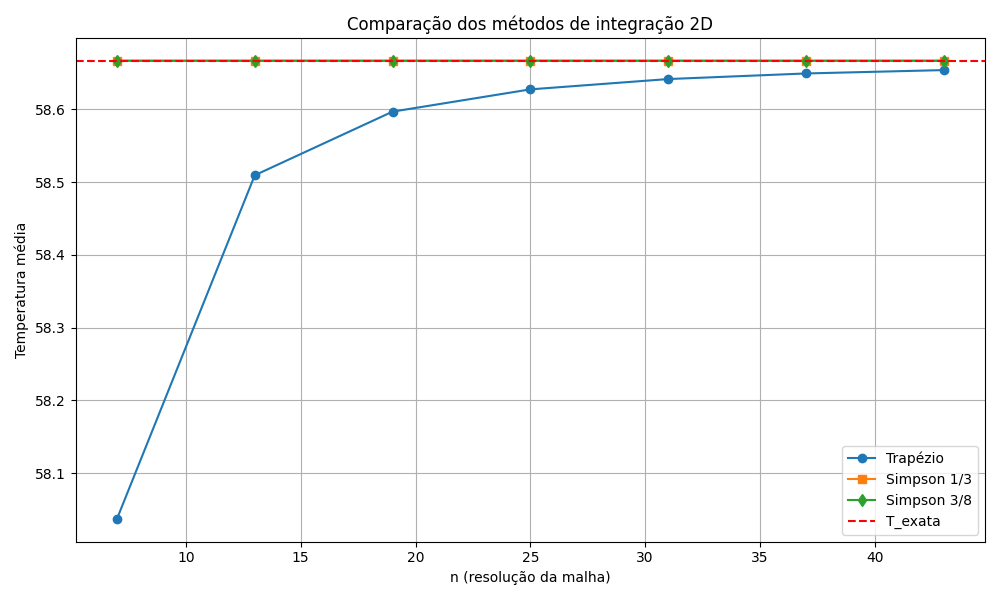
\includegraphics[width=0.8\textwidth]{img/Figure_1.png}
    \caption{Gráfico comparativo dos erros absolutos dos métodos de integração numérica.}
\end{figure}

\section{Estrutura do Código}

\subsection*{Trecho principal}

\begin{lstlisting}[language=Python, caption={Funcao principal que executa os calculos e organiza os resultados.}]
# Trecho central do codigo (trechos omitidos por brevidade)
import numpy as np
import pandas as pd
import matplotlib.pyplot as plt

# === CONFIGURACOES GERAIS ===
T_EXATA = 58.6666666666667
ARQUIVO_MALHAS = "malhas_T.txt"
valores_n = [7, 13, 19, 25, 31, 37, 43]

# === FUNCAO T(x, y) ===
def T(x, y):
    return 2*x*y + 2*x - x**2 - 2*y**2 + 72

# === ETAPA 1: GERAR ARQUIVO DE MALHAS ===
def gerar_arquivo_malhas(nome_arquivo):
    with open(nome_arquivo, 'w') as f:
        f.write("n\tx\ty\tT(x,y)\tErro_Absoluto\n")
        for n in valores_n:
            x_vals = np.linspace(0, 8, n)
            y_vals = np.linspace(0, 6, n)
            X, Y = np.meshgrid(x_vals, y_vals, indexing='ij')
            T_vals = T(X, Y)
            erro = abs(np.mean(T_vals) - T_EXATA)
            for i in range(n):
                for j in range(n):
                    f.write(f"{n}\t{X[i,j]:.4f}\t{Y[i,j]:.4f}\t{T_vals[i,j]:.4f}\t{erro:.6f}\n")
    print(f"[OK] Arquivo '{nome_arquivo}' gerado.")

# === ETAPA 2: LER O ARQUIVO E ORGANIZAR AS MALHAS ===
def ler_malhas_do_txt(arquivo):
    data = pd.read_csv(arquivo, sep='\t')
    grupos = {}
    for n in data['n'].unique():
        grupo = data[data['n'] == n]
        n_int = int(n)
        x_vals = grupo['x'].values.reshape((n_int, n_int))
        y_vals = grupo['y'].values.reshape((n_int, n_int))
        T_vals = grupo['T(x,y)'].values.reshape((n_int, n_int))
        grupos[n_int] = {'x': x_vals, 'y': y_vals, 'T': T_vals}
    return grupos

# === METODO: TRAPEZIO 2D ===
def integrar_trapezio_2d(T, a, b, c, d):
    n, m = T.shape
    hx = (b - a) / (n - 1)
    hy = (d - c) / (m - 1)
    total = 0
    for i in range(n):
        for j in range(m):
            peso = 1
            if i in [0, n-1]: peso *= 0.5
            if j in [0, m-1]: peso *= 0.5
            total += peso * T[i, j]
    return (hx * hy * total) / ((b - a) * (d - c))

# === METODO: SIMPSON 1/3 2D ===
def integrar_simpson_1_3_2d(T, a, b, c, d):
    n, m = T.shape
    if (n - 1) % 2 != 0 or (m - 1) % 2 != 0:
        return np.nan  # Nao aplicavel
    hx = (b - a) / (n - 1)
    hy = (d - c) / (m - 1)
    total = 0
    for i in range(n):
        for j in range(m):
            coef_x = 4 if i % 2 != 0 else 2
            coef_y = 4 if j % 2 != 0 else 2
            if i in [0, n-1]: coef_x = 1
            if j in [0, m-1]: coef_y = 1
            total += coef_x * coef_y * T[i, j]
    integral = (hx * hy / 9) * total
    return integral / ((b - a) * (d - c))

# === METODO: SIMPSON 3/8 2D ===
def integrar_simpson_3_8_2d(T, a, b, c, d):
    n, m = T.shape
    if (n - 1) % 3 != 0 or (m - 1) % 3 != 0:
        return np.nan  # Nao aplicavel
    hx = (b - a) / (n - 1)
    hy = (d - c) / (m - 1)
    total = 0
    for i in range(n):
        for j in range(m):
            if i == 0 or i == n - 1:
                coef_x = 1
            elif i % 3 == 0:
                coef_x = 2
            else:
                coef_x = 3

            if j == 0 or j == m - 1:
                coef_y = 1
            elif j % 3 == 0:
                coef_y = 2
            else:
                coef_y = 3

            total += coef_x * coef_y * T[i, j]
    integral = (3 * hx * 3 * hy / 64) * total
    return integral / ((b - a) * (d - c))

# === ETAPA 4: CALCULO DAS TEMPERATURAS E ERROS ===
def calcular_temperaturas_medias(grupos, T_exata):
    resultados = []
    for n, dados in grupos.items():
        Tmat = dados['T']
        t_trap = integrar_trapezio_2d(Tmat, 0, 8, 0, 6)
        t_simp_1_3 = integrar_simpson_1_3_2d(Tmat, 0, 8, 0, 6)
        t_simp_3_8 = integrar_simpson_3_8_2d(Tmat, 0, 8, 0, 6)
        resultados.append({
            'n': n,
            'T_trapezio': t_trap,
            'Erro_trapezio': abs(t_trap - T_exata),
            'T_simpson_1_3': t_simp_1_3,
            'Erro_simp_1_3': abs(t_simp_1_3 - T_exata) if not np.isnan(t_simp_1_3) else np.nan,
            'T_simpson_3_8': t_simp_3_8,
            'Erro_simp_3_8': abs(t_simp_3_8 - T_exata) if not np.isnan(t_simp_3_8) else np.nan
        })
    return pd.DataFrame(resultados).sort_values(by='n')

# === ETAPA 5: PLOTAGEM FINAL ===
def plotar_resultado(df):
    plt.figure(figsize=(10,6))
    plt.plot(df['n'], df['T_trapezio'], 'o-', label='Trapezio')
    plt.plot(df['n'], df['T_simpson_1_3'], 's-', label='Simpson 1/3')
    plt.plot(df['n'], df['T_simpson_3_8'], 'd-', label='Simpson 3/8')
    plt.axhline(y=T_EXATA, color='r', linestyle='--', label='T_exata')
    plt.xlabel('n (resolucao da malha)')
    plt.ylabel('Temperatura media')
    plt.title('Comparacao dos metodos de integracao 2D')
    plt.legend()
    plt.grid(True)
    plt.tight_layout()
    plt.show()

# === EXECUCAO PRINCIPAL ===
if __name__ == "__main__":
    gerar_arquivo_malhas(ARQUIVO_MALHAS)
    grupos = ler_malhas_do_txt(ARQUIVO_MALHAS)
    df_result = calcular_temperaturas_medias(grupos, T_EXATA)

    # Exibir tabela com os erros
    print("\nTabela de Resultados:")
    print(df_result.to_string(index=False, float_format='{:0.6f}'.format))

    # Plotar grafico comparativo
    plotar_resultado(df_result)

\end{lstlisting}

\subsection*{Funções auxiliares}

\begin{itemize}
  \item \textbf{Regra do Trapézio:} Implementada como somatório ponderado de bordas, intermediários e cantos.
  \item \textbf{Regra 1/3 de Simpson:} Usa somas alternadas com pesos 4 e 2 para linhas ímpares e pares.
  \item \textbf{Regra 3/8 de Simpson:} Aplica-se sobre subconjuntos de 4 pontos por linha/coluna. Exige que o número de nós seja múltiplo de 3.
\end{itemize}

\subsection*{Geração de Gráficos}

Os valores médios $\bar{T}$ para cada método são armazenados em listas e representados graficamente em função do número de nós $n$. A curva do valor exato também é plotada para comparação visual dos erros.

\end{document}